% resume.tex
%
% Omid Mashayekhi

\documentclass[letterpaper,10pt]{article}

%-----------------------------------------------------------
\usepackage{enumitem}
\usepackage{graphicx}
\usepackage{textpos}
\usepackage{ifthen}
\usepackage[empty]{fullpage}
\usepackage[colorlinks=true, urlcolor=blue]{hyperref}
\raggedbottom
\raggedright
\setlength{\tabcolsep}{0in}

% Adjust margins to 0.5in on all sides
\addtolength{\oddsidemargin}{-0.5in}
\addtolength{\evensidemargin}{-0.5in}
\addtolength{\topmargin}{-0.5in}
\addtolength{\textheight}{1.0in}
\addtolength{\textwidth}{1.0in}

%-----------------------------------------------------------
%Custom commands

\newcommand{\heading}[1] {
  {\large
    \begin{minipage}
    {\textwidth}
    {\textbf{#1}}
    \end{minipage}
  }
  \begin{center}
  \vspace{-15pt}
  \line(1,0){520}
  \end{center}
}


\newcommand{\template}[2]{
\begin{tabular*}{7.0in}{l@{\extracolsep{\fill}}r}
		#1 & \textit{#2} \\
\end{tabular*}\vspace{-1pt}}


\usepackage{catchfile}
\newcommand{\getenv}[2]{%
  \CatchFileEdef{\temp}{"|kpsewhich --var-value #2"}{}%
  \if\relax\detokenize{#1}\relax\temp\else\let#1\temp\fi}

\getenv{\ISEXTENDED}{ISEXTENDED}

%-----------------------------------------------------------


\begin{document}

\centering

\textbf{\LARGE Omid Mashayekhi}

\setlength{\TPHorizModule}{10pt} %controls horizontal movements
\setlength{\TPVertModule}{10pt}  %controls vertical movements

\begin{textblock}{4}(1,0)
\begin{tabular}{lr}
\textbf{Address:}    & Menlo Park, CA\\
\textbf{Website:}    & ~~\href{http://www.omidm.net}{\url{www.omidm.net}}\\
\end{tabular}
\end{textblock}

\begin{textblock}{4}(37,0)
\begin{tabular}{lr}
\textbf{E-Mail:}     & 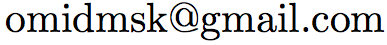
\includegraphics[width=1.2in]{figs/gmail.png}\\
\textbf{Cell Phone:} & 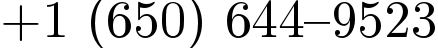
\includegraphics[width=1in]{figs/cell-phone.png}\\
\end{tabular}
\end{textblock}

\vspace{30pt}





\heading{Education}

\begin{tabular*}{7.0in}{l@{\extracolsep{\fill}}r}
\textbf{\large Stanford University}  & Stanford, CA \\
~~~\textbf{Ph.D.} in Electrical Engineering, Cloud Computing    & Winter 2013 - Spring 2017\\
~~~\textbf{Ph.D. Minor} in Computer Science, Systems Track       & Winter 2013 - Spring 2017\\
~~~\textbf{M.Sc.} in Electrical Engineering, Networking Systems & Fall 2011 - Spring 2013\\
\end{tabular*}

\vspace{5pt}

\begin{tabular*}{7.0in}{l@{\extracolsep{\fill}}r}
\textbf{Sharif University of Technology} & Tehran, Iran\\
~~~\textbf{B.Sc.} in Electrical Engineering, Communication Systems & Fall 2007 - Spring 2011\\
\end{tabular*}

\vspace{5pt}





\heading{Experience}

\begin{tabular*}{7.0in}{l@{\extracolsep{\fill}}r}
\textbf{Staff Software Engineer at Google}  & Mountain View, CA \\
~~~NetInfra, developing distributed software systems for networking applications. &  Summer 2017 - Present\\
\end{tabular*}

\vspace{5pt}

\begin{tabular*}{7.0in}{l@{\extracolsep{\fill}}r}
\textbf{Software Engineer Intern at bebop Inc.}  & Los Altos, CA \\
~~~Back-end engineer working on developing a low latency data store. &  Summer 2015\\
\end{tabular*}

\vspace{5pt}

\begin{tabular*}{7.0in}{l@{\extracolsep{\fill}}r}
\textbf{RA at Stanford Information Networks Group (SING)}  & Stanford University\\
~~~Diverse projects from cloud computing and graphical simulations to full duplex radio. & Fall 2011 - Spring 2017\\
\end{tabular*}
	
\vspace{5pt}

\begin{tabular*}{7.0in}{l@{\extracolsep{\fill}}r}
\textbf{Software Engineer Intern at Cisco Systems }  & San Jose, CA \\
~~~Software engineer at Wireless Networking Business Unit (WNBU). & Summer 2012 \\
\end{tabular*}
	
\vspace{5pt}

\ifthenelse{\equal{\ISEXTENDED}{true }}{

\begin{tabular*}{7.0in}{l@{\extracolsep{\fill}}r}
\textbf{Teaching Experience} & Stanford University \\
~~~Course Assistant in CS344C, Cloud Simulation Systems. & Spring 2013 \\
\end{tabular*}
	
\vspace{5pt}

\begin{tabular*}{7.0in}{l@{\extracolsep{\fill}}r}
\textbf{RA at Advanced Communications Research Institute (ACRI) }  & Sharif University \\
~~~Research in power estimation and coding techniques for CDMA systems & Spring 2009 - Summer 2011 \\
\end{tabular*}
	
\vspace{5pt}

}{} % End If




\heading{Selected Projects}

\begin{itemize}[noitemsep,topsep=0pt, leftmargin=.5cm, rightmargin=.5cm]


\item[]
\href{https://research.google/pubs/pub51587/}{\textbf{Jupiter:}}
Google's data center networking technology with traffic and topology enginering trhough SDN.


\vspace{5pt}

\item[]
\href{http://nimbus.stanford.edu}{\textbf{Nimbus:}}
a cloud computing framework for fast data analytics and HPC applications.

\ifthenelse{\equal{\ISEXTENDED}{true }}{

\vspace{5pt}

\item[]
\textbf{Janus:}
centralized MAC protocol for full duplex radio that realizes double capacity.

\vspace{5pt}

\item[]
\textbf{Predicting x86 Runtime:}
supervised learning algorithms to predict serialized x86 programs runtime. 

\vspace{5pt}

\item[]
\textbf{Packet Classification in Presence of Wildcard:}
scalable, memory efficient, software-based algorithm.

\vspace{5pt}

\item[]
\textbf{OpenFlow Controller for DCell:}
simulating DCell topology for data centers using Mininet OpenFlow controller.

}{} % End If

\end{itemize}

\vspace{5pt}




\heading{Selected Papers}

\begin{itemize}[noitemsep,topsep=0pt, leftmargin=.5cm, rightmargin=.5cm]

\item[]
L. Poutievski, \textbf{O. Mashayekhi}, J. Ong, A. Singh, M. Tariq, R. Wang,
J. Zhang, V. Beauregard, P. Conner, S. Gribble, R. Kapoor, S. Kratzer,
N. Li, H. Liu, K. Nagaraj, J. Ornstein, S. Sawhney, R. Urata, L. Vicisano,
K. Yasumura, S. Zhang, J. Zhou, A. Vahdat
"Jupiter Evolving: Transforming Google's Datacenter Network via Optical Circuit Switches and Software-Defined Networking",
In Proceedings of ACM SIGCOMM 2022.

\vspace{5pt}

\item[]
\textbf{O. Mashayekhi}, C. Shah, H. Qu, A. Lim, P. Levis
"Automatically Distributing Eulerian and Hybrid Fluid Simulations in the Cloud",
In ACM Transactions on Graphics, vol. 37, no. 2, Article 24, June 2018, Presented at SIGGRAPH 2018.

\vspace{5pt}

\item[]
\textbf{O. Mashayekhi}, H. Qu, C. Shah, P. Levis
"Execution Templates: Caching Control Plane Decisions for Strong Scaling of Data Analytics",
In proceedings of 2017 USENIX Annual Technical Conference (USENIX ATC '17).

\ifthenelse{\equal{\ISEXTENDED}{true }}{

\vspace{5pt}

\item[]
H. Qu, \textbf{O. Mashayekhi}, C. Shah, P. Levis
"Decoupling the Control Plane from Program Control Flow for Flexibility and Performance in Cloud Computing",
In Proceedings of the 13th European Conference on Computer Systems (EuroSys '18), 2018

\vspace{5pt}

\item[]
J. Y. Kim, \textbf{O. Mashayekhi}, H. Qu, M. Kazandjieva, and P. Levis,
"Janus: A Novel MAC Protocol for Full Duplex Radio",
Stanford CSTR 2013-02, 2013.

\vspace{5pt}

\item[]
\textbf{O. Mashayekhi}, and F. Marvasti,
"Uniquely Decodable Codes with Fast Decoder for Overloaded Synchronous CDMA Systems",
In IEEE Transactions on Communication, vol. 60, no. 11, pp. 3145-3149, November 2012.

}{} % End If

\end{itemize}

\vspace{5pt}





\heading{Patents}

\begin{itemize}[noitemsep,topsep=0pt, leftmargin=.5cm, rightmargin=.5cm]
\item[]
\textbf{O. Mashayekhi}, and F. Marvasti,
"Uniquely Decodable Codes and Decoder for Overloaded Synchronous CDMA Systems",
US Patent 8,582,604, 2013
\end{itemize}

\vspace{5pt}





% \ifthenelse{\equal{\ISEXTENDED}{true }}{\break}{}

\heading{Computer Skills}

\begin{description}

\item[~~~~~Programming Languages:]
C++, C, Python, Java, JavaScript, Shell script, Ruby, Assembly.

\item[~~~~~Systems and Softwares:]
Apache Spark, Naiad, Mininet, MATLAB, MATHCAD

\end{description}





\heading{Selected Honors and Awards}

\begin{itemize}

\item \template{Recipient of Google Feats of Engineering Award.}{2018}

\item \template{Recipient of 2-year Stanford Graduate Fellowship (Cisco Systems Fellow).}{2013-2015}

\item \template{Ranked $15^{th}(/135)$ in the EE Qualifying Examination, Stanford University.}{2013}

\item \template{Ranked $2^{nd}$ in the EE Depart., Comm. branch, Sharif University of Technology.}{Class of 2007-2011}

\item \template{Bronze medalist of Iran National Mathematics Olympiad.}{2006}

\ifthenelse{\equal{\ISEXTENDED}{true }}{

\item \template{Second winner of the "Bests Undergraduate Thesis Award", Sharif University of Technology.}{2011}

\item \template{Ranked $46^{th}$ in university entrance exam among more than 300,000 students.}{2007}

}{} % End If

\end{itemize}





\heading{Extracurricular Activities}

\begin{description}

\item[~~~~~] Social Ballroom Dancing, Playing Tennis, Golfing, Swimming, Travelling.

\end{description}


\end{document}
